%  LaTeX support: latex@mdpi.com 
%  For support, please attach all files needed for compiling as well as the log file, and specify your operating system, LaTeX version, and LaTeX editor.

%=================================================================
\documentclass[biomimetics,article,submit,pdftex,moreauthors]{Definitions/mdpi} 
%\documentclass[preprints,article,submit,pdftex,moreauthors]{Definitions/mdpi} 
% For posting an early version of this manuscript as a preprint, you may use "preprints" as the journal. Changing "submit" to "accept" before posting will remove line numbers.

% Below journals will use APA reference format:
% admsci, aieduc, behavsci, businesses, econometrics, economies, education, ejihpe, famsci, games, humans, ijcs, ijfs, jintelligence, journalmedia, jrfm, jsam, languages, peacestud, psycholint, publications, tourismhosp, youth

% Below journals will use Chicago reference format:
% arts, genealogy, histories, humanities, laws, literature, religions, risks, socsci

%--------------------
% Class Options:
%--------------------
%----------
% journal
%----------
% Choose between the following MDPI journals:

%---------
% article
%---------
% The default type of manuscript is "article", but can be replaced by: 
% abstract, addendum, article, benchmark, book, bookreview, briefcommunication, briefreport, casereport, changes, clinicopathologicalchallenge, comment, commentary, communication, conceptpaper, conferenceproceedings, correction, conferencereport, creative, datadescriptor, discussion, entry, expressionofconcern, extendedabstract, editorial, essay, erratum, fieldguide, hypothesis, interestingimages, letter, meetingreport, monograph, newbookreceived, obituary, opinion, proceedingpaper, projectreport, reply, retraction, review, perspective, protocol, shortnote, studyprotocol, supfile, systematicreview, technicalnote, viewpoint, guidelines, registeredreport, tutorial,  giantsinurology, urologyaroundtheworld
% supfile = supplementary materials

%----------
% submit
%----------
% The class option "submit" will be changed to "accept" by the Editorial Office when the paper is accepted. This will only make changes to the frontpage (e.g., the logo of the journal will get visible), the headings, and the copyright information. Also, line numbering will be removed. Journal info and pagination for accepted papers will also be assigned by the Editorial Office.

%------------------
% moreauthors
%------------------
% If there is only one author the class option oneauthor should be used. Otherwise use the class option moreauthors.

%---------
% pdftex
%---------
% The option pdftex is for use with pdfLaTeX. Remove "pdftex" for (1) compiling with LaTeX & dvi2pdf (if eps figures are used) or for (2) compiling with XeLaTeX.

%=================================================================
% MDPI internal commands - do not modify
\firstpage{1} 
\makeatletter 
\setcounter{page}{\@firstpage} 
\makeatother
\pubvolume{1}
\issuenum{1}
\articlenumber{0}
\pubyear{2026}
\copyrightyear{2026}
%\externaleditor{Firstname Lastname} % More than 1 editor, please add `` and '' before the last editor name
\datereceived{ } 
\daterevised{ } % Comment out if no revised date
\dateaccepted{ } 
\datepublished{ } 
%\datecorrected{} % For corrected papers: "Corrected: XXX" date in the original paper.
%\dateretracted{} % For retracted papers: "Retracted: XXX" date in the original paper.
%\doinum{} % Used for some special journals, like molbank
%\pdfoutput=1 % Uncommented for upload to arXiv.org
%\CorrStatement{yes}  % For updates
%\longauthorlist{yes} % For many authors that exceed the left citation part
%\IsAssociation{yes} % For association journals

%=================================================================
% Add packages and commands here. The following packages are loaded in our class file: fontenc, inputenc, calc, indentfirst, fancyhdr, graphicx, epstopdf, lastpage, ifthen, float, amsmath, amssymb, lineno, setspace, enumitem, mathpazo, booktabs, titlesec, etoolbox, tabto, xcolor, colortbl, soul, multirow, microtype, tikz, totcount, changepage, attrib, upgreek, array, tabularx, pbox, ragged2e, tocloft, marginnote, marginfix, enotez, amsthm, natbib, hyperref, cleveref, scrextend, url, geometry, newfloat, caption, draftwatermark, seqsplit
% cleveref: load \crefname definitions after \begin{document}

%=================================================================
% Please use the following mathematics environments: Theorem, Lemma, Corollary, Proposition, Characterization, Property, Problem, Example, ExamplesandDefinitions, Hypothesis, Remark, Definition, Notation, Assumption
%% For proofs, please use the proof environment (the amsthm package is loaded by the MDPI class).

%=================================================================
\usepackage{tikz}
\usetikzlibrary{arrows.meta,positioning,fit,calc,shapes.geometric,shapes.misc}

\usepackage{xcolor}
\usepackage{manyfoot}

%% Standard packages
%\usepackage{graphicx}
%\usepackage{booktabs}
%\usepackage{multirow}
\usepackage{amsmath,amssymb}
\usepackage{enumitem}
\usepackage{algorithm}
\usepackage{algpseudocode}
%\usepackage{url}
%% Local macros
\newcommand{\model}{V-CHIMERA}
\newcommand{\igc}{Immune-Gated Coupling (IGC)}
\newcommand{\envname}{CyberCrisisGym-J}

% Full title of the paper (Capitalized)
\Title{Immune-Inspired Verified Coupled Human--Information--Machine Incident Response for Misinformation-Aware Cyber Defense}

% Author Orchid ID: enter ID or remove command
\newcommand{\orcidauthorA}{0000-0002-2111-3456} % Add \orcidA{} behind the author's name
%\newcommand{\orcidauthorB}{0000-0000-0000-000X} % Add \orcidB{} behind the author's name

% Authors, for the paper (add full first names)
\Author{Fahad Alghamdi\orcidA{} and Saad Alqithami*\orcidB{}}

}

%\longauthorlist{yes}

% MDPI internal command: Authors, for metadata in PDF
\AuthorNames{Fahad Alghamdi, Saad Alqithami}

%\longauthorlist{yes}

% Affiliations / Addresses (Add [1] after \address if there is only one affiliation.)
\address{Computer Science Department, Al-Baha University, Albaha 65779, Saudi Arabia.}

% Contact information of the corresponding author
\corres{Correspondence: salqithami@bu.edu.sa}

% Current address and/or shared authorship
%\firstnote{Current address: Affiliation.}  
% Current address should not be the same as any items in the Affiliation section.

%\secondnote{These authors contributed equally to this work.}
% The commands \thirdnote{} till \eighthnote{} are available for further notes.

%\simplesumm{} % Simple summary

%\conference{} % An extended version of a conference paper

% Abstract (Do not insert blank lines, i.e. \\) 
\abstract{In cyber crises, incident response increasingly depends on coupled cyber operations and public communication, yet these two control loops are often engineered and governed in isolation. We present \model{}, an integrated cyber--social incident response framework that explicitly models how misinformation, trust, and polarization interact with cyber-defense actions. Our contribution is threefold: (i) a verified coupling architecture that links cyber state, social belief dynamics, and response actions; (ii) a protocol-enforcing communication shield that guarantees zero executed violations while logging attempted unsafe actions; and (iii) an immune-gated coupling (IGC) controller inspired by immune tolerance and danger signaling, which escalates coupling and counter-messaging only when evidence warrants it. Across three representative crisis scenarios (ransomware rumor, service outage rumor, and exfiltration scam), we find that naive coupling can be brittle, but IGC improves the cyber--social trade-off (lower cyber harm and misbelief, higher or preserved trust) under protocol safety. Sensitivity analysis further shows that IGC attenuates the degradation observed under strong coupling and weak platform moderation.}

% Keywords
\keyword{cyber incident response; crisis communication; misinformation; social cybersecurity; biomimetics; artificial immune systems; danger theory; multi-agent systems; runtime enforcement; socio-technical risk}

% The fields PACS, MSC, and JEL may be left empty or commented out if not applicable
%\PACS{J0101}
%\MSC{}
%\JEL{}

%%%%%%%%%%%%%%%%%%%%%%%%%%%%%%%%%%%%%%%%%%
% Only for the journal Diversity
%\LSID{\url{http://}}

%%%%%%%%%%%%%%%%%%%%%%%%%%%%%%%%%%%%%%%%%%
% Only for the journal Applied Sciences
%\featuredapplication{Authors are encouraged to provide a concise description of the specific application or a potential application of the work. This section is not mandatory.}
%%%%%%%%%%%%%%%%%%%%%%%%%%%%%%%%%%%%%%%%%%

%%%%%%%%%%%%%%%%%%%%%%%%%%%%%%%%%%%%%%%%%%
% Only for the journal Data
%\dataset{DOI number or link to the deposited data set if the data set is published separately. If the data set shall be published as a supplement to this paper, this field will be filled by the journal editors. In this case, please submit the data set as a supplement.}
%\datasetlicense{License under which the data set is made available (CC0, CC-BY, CC-BY-SA, CC-BY-NC, etc.)}

%%%%%%%%%%%%%%%%%%%%%%%%%%%%%%%%%%%%%%%%%%
% Only for the journal BioTech, Fishes, Neuroimaging and Toxins
%\keycontribution{The breakthroughs or highlights of the manuscript. Authors can write one or two sentences to describe the most important part of the paper.}

%%%%%%%%%%%%%%%%%%%%%%%%%%%%%%%%%%%%%%%%%%
% Only for the journal Encyclopedia
%\encyclopediadef{For entry manuscripts only: please provide a brief overview of the entry title instead of an abstract.}

%%%%%%%%%%%%%%%%%%%%%%%%%%%%%%%%%%%%%%%%%%
% Different journals have different requirements. Please check the specific journal guidelines in the "Instructions for Authors" on the journal's official website.
%\addhighlights{yes}
%\renewcommand{\addhighlights}{%
%
%\noindent The goal is to increase the discoverability and readability of the article via search engines and other scholars. Highlights should not be a copy of the abstract, but a simple text allowing the reader to quickly and simplified find out what the article is about and what can be cited from it. Each of these parts should be devoted up to 2~bullet points.\vspace{3pt}\\
%\textbf{What are the main findings?}
% \begin{itemize}[labelsep=2.5mm,topsep=-3pt]
% \item First bullet.
% \item Second bullet.
% \end{itemize}\vspace{3pt}
%\textbf{What are the implications of the main findings?}
% \begin{itemize}[labelsep=2.5mm,topsep=-3pt]
% \item First bullet.
% \item Second bullet.
% \end{itemize}
%}

%%%%%%%%%%%%%%%%%%%%%%%%%%%%%%%%%%%%%%%%%%

\providecommand{\bibcommenthead}[1]{}

\begin{document}

\section{Introduction}
Cyber incidents are rarely confined to technical containment. Ransomware disruptions, service outages, and data-exfiltration events are routinely accompanied by rumor, speculation, coordinated disinformation, and opportunistic scams, all of which can shape public behavior and constrain operational response. This aligns with the literature on \emph{social cybersecurity}, which emphasizes that human behavior and online information flows are integral to cybersecurity outcomes \citep{carley2020social,mulahuwaish2025survey}.

From an incident-response perspective, misinformation can \emph{increase} harm by suppressing reporting of indicators, discouraging compliance with mitigation guidance, overwhelming helpdesks, or redirecting victims to follow-on phishing and fraud. Conversely, crisis communications are safety-critical: overconfident debunks, premature attribution, or over-disclosure can cause irreversible damage (panic, legal exposure, privacy breaches, or loss of trust). Despite these bidirectional dependencies, autonomous cyber-defense benchmarks typically study containment in isolation (e.g., enterprise-defense simulation gyms \citep{baillie2020cyborg,kunz2023multiagent}), while misinformation research often evaluates interventions without closed-loop operational feedback \citep{lazer2018science,vosoughi2018spread,kozyreva2024toolbox,lewandowsky2021inoculation,ng2021platform}.

This paper asks how to design socio-technical decision systems that \emph{jointly} manage incident response and public communication under explicit governance constraints. We focus on three research questions:
\begin{enumerate}[leftmargin=*]
  \item \textbf{RQ1:} When public sentiment affects operational dynamics, does coupling sentiment into incident-response decision-making improve outcomes under misinformation?
  \item \textbf{RQ2:} When messaging capacity is limited and susceptibility is heterogeneous, do targeted counter-messaging strategies better reduce misbelief and preserve trust than non-targeted baselines?
  \item \textbf{RQ3:} Can runtime protocol enforcement eliminate unsafe communications (zero executed violations) while preserving effectiveness?
\end{enumerate}

\subsection{Contributions}
We make five contributions:
\begin{enumerate}[leftmargin=*]
  \item \textbf{Problem formulation.} We formalize misinformation-aware incident response as a constrained partially observable stochastic game (C-POSG) with a coupled cyber--social state and a safety-constrained communication channel.
  \item \textbf{Verified architecture.} We introduce \model{}, a modular two-agent decision architecture coupling cyber operations and crisis communication through a shared belief-state estimate and an explicit coupling function.
  \item \textbf{Bio-inspired coupling control.} We propose \igc{}, an immune-inspired regulator that gates when the controller relies on cyber--social feedback using a cyber ``danger'' signal and social uncertainty, and scales targeted counter-messaging using antigen scores with short-term memory.
  \item \textbf{Runtime enforcement for communication safety.} We adapt shielding to crisis messaging by enforcing protocol predicates at runtime, guaranteeing zero executed protocol violations and producing auditable intervention logs.
  \item \textbf{Reproducible testbed and evaluation.} We instantiate the framework in \envname{} and report scenario-based experiments with ablations and sensitivity analysis in a fully scriptable pipeline.
\end{enumerate}

\section{Background and related work}
We situate \model{} at the intersection of misinformation dynamics, social cybersecurity, multi-agent decision-making, and safe runtime enforcement.

\subsection{Misinformation dynamics and interventions}
False information can spread faster and farther than corrections in online networks \citep{vosoughi2018spread,lazer2018science}. Susceptibility is shaped by attention and reasoning constraints \citep{pennycook2019lazy}. Interventions such as debunking, prebunking/inoculation, accuracy prompts, and platform moderation can reduce belief and sharing of falsehoods \citep{kozyreva2024toolbox,lewandowsky2021inoculation,ng2021platform}. In crisis settings, however, interventions are embedded in operational feedback loops: public compliance and reporting affect incident evolution, and cyber events (confirmed breach, service loss) shift beliefs and trust. This motivates closed-loop evaluation rather than isolated intervention assessment.

\subsection{Opinion dynamics and social-network models}
Opinion dynamics models provide mechanistic abstractions for belief evolution under social influence, including DeGroot consensus \citep{degroot1974reaching} and bounded confidence \citep{hegselmann2002opinion}. We adopt an agent-based modeling approach because cyber--social crises are heterogeneous, multi-platform, and adversarially manipulated (bots and coordinated campaigns). The \envname{} social backend exposes interpretable parameters (susceptibility, correction efficacy, moderation strength) and yields macro metrics including misbelief, trust, uncertainty, and polarization.

\subsection{Social cybersecurity and cyber--social coupling}
Social cybersecurity argues that attackers exploit both technical and social channels \citep{carley2020social,mulahuwaish2025survey}. In incident response, public behavior affects detection (e.g., user-reported phishing) and mitigation (compliance with patching and isolation guidance). Our framework encodes these dependencies via an explicit coupling function and evaluates policy trade-offs under different coupling regimes.

\subsection{Multi-agent systems and coordination under uncertainty}
Multi-agent systems provide tools for distributed decision-making and coordination under uncertainty \citep{wooldridge2009introduction,jennings2001agentbased,rahwan2019machine,tambe2011security}. In cyber defense, simulation environments such as CybORG \citep{baillie2020cyborg} and CyberBattleSim \citep{kunz2023multiagent} enable evaluation of autonomous defenders, but typically omit the public communication dimension and associated safety constraints.

\subsection{Safe decision-making and shielding}
Runtime shielding can prevent unsafe actions during learning or deployment by enforcing hard constraints on the executed policy \citep{alshiekh2018safe,koenighofer2024shields}. We adapt this concept to \emph{communication safety} in cyber crises: unsafe actions correspond to protocol violations such as over-claiming without evidence, over-disclosure of sensitive details, or harmful user instructions. Because communications can create irreversible harm, hard constraints are appropriate.


\subsection{Bio-inspired defense and artificial immune systems}
Biological immune systems offer a canonical example of distributed defense under uncertainty: they detect pathogens through imperfect signals, allocate limited resources between detection and response, and regulate responses to avoid collateral damage.
Artificial immune systems (AIS) and danger-theory-inspired models translate these principles into anomaly detection and adaptive control mechanisms, often emphasizing the role of \emph{danger signals} (contextual evidence of harm) rather than pattern matching alone \citep{matzinger1994tolerance,greensmith2005dendritic,decastro2002artificial}.
We leverage this perspective to motivate an immune-inspired regulator for cyber--social coupling in \model{}.
Concretely, we treat incident severity and evidence quality as a \emph{danger signal}, treat community sentiment risks as an \emph{antigen load} with short-term memory, and use these signals to (i) gate when the cyber controller relies on social-to-cyber feedback and (ii) scale the intensity and targeting of counter-messaging (Section~\ref{sec:igc}).
The protocol shield functions as a conservative \emph{checkpoint}: even under high activation, unsafe communications are prevented from executing and are logged for auditability, reducing the risk of ``autoimmune'' overreaction.

Our sensitivity analysis (Section~\ref{sec:sensitivity}) can be interpreted as a calibration study: stronger cyber--social coupling increases the operational consequence of misinformation, while platform moderation acts as an external filter that attenuates exposure.

\section{Research design}
We follow a design science perspective \citep{hevner2004designscience,peffers2007dsrm}, treating \model{} as a socio-technical artifact for cyber crisis management in online information environments. Design science is appropriate because the contribution is prescriptive: we build a verified decision architecture and evaluate its utility under controlled conditions.

The design objectives are: (i) explicitly model cyber--social coupling; (ii) support targeted counter-messaging under heterogeneous diffusion; (iii) enforce non-negotiable communication protocol constraints via runtime enforcement; and (iv) provide transparent evaluation and artifact transparency. We evaluate \model{} in \envname{} using scenario-based simulation, ablations (no coupling, no targeting), and baseline pipelines with and without shielding.

\section{Problem formulation}
We model a misinformation-aware cyber crisis as a constrained partially observable stochastic game.

\subsection{State, actions, and observations}
Let $s_t = (s^C_t, s^S_t)$ denote the joint state at time $t$, comprising cyber state $s^C_t$ (e.g., compromise status and service availability) and social state $s^S_t$ (distribution of beliefs and trust across a population and platforms). Two decision-makers act at each step: a cyber agent with action $a^C_t \in \mathcal{A}^C$ (operational response such as isolation, patching, restoration, and detection), and a communication agent with action $a^M_t \in \mathcal{A}^M$ (public messaging such as status updates, advisories, or rumor corrections).

Observations are partial: $o^C_t$ captures noisy cyber telemetry, while $o^S_t$ captures noisy social signals (polls, sentiment summaries, or sampled posts). Agents may share a belief state $b_t \approx p(s_t \mid o_{\le t}, a_{<t})$.

\subsection{Objectives and constraints}
We seek to reduce cyber harm while stabilizing sentiment:
\begin{align}
R_t &= -\alpha \cdot H(s^C_t) - \beta \cdot M(s^S_t) + \gamma \cdot T(s^S_t),
\end{align}
where $H$ is cyber harm (e.g., service loss and exfiltration), $M$ is misbelief, and $T$ is trust. Communication safety constraints are encoded as protocol predicates $g_k(s_t,a^M_t) \le 0$. A runtime shield enforces these constraints by editing unsafe actions into safe alternatives.

\section{\model{} framework}
Figure~\ref{fig:arch} summarizes the architecture.

\begin{figure*}[t]
\centering
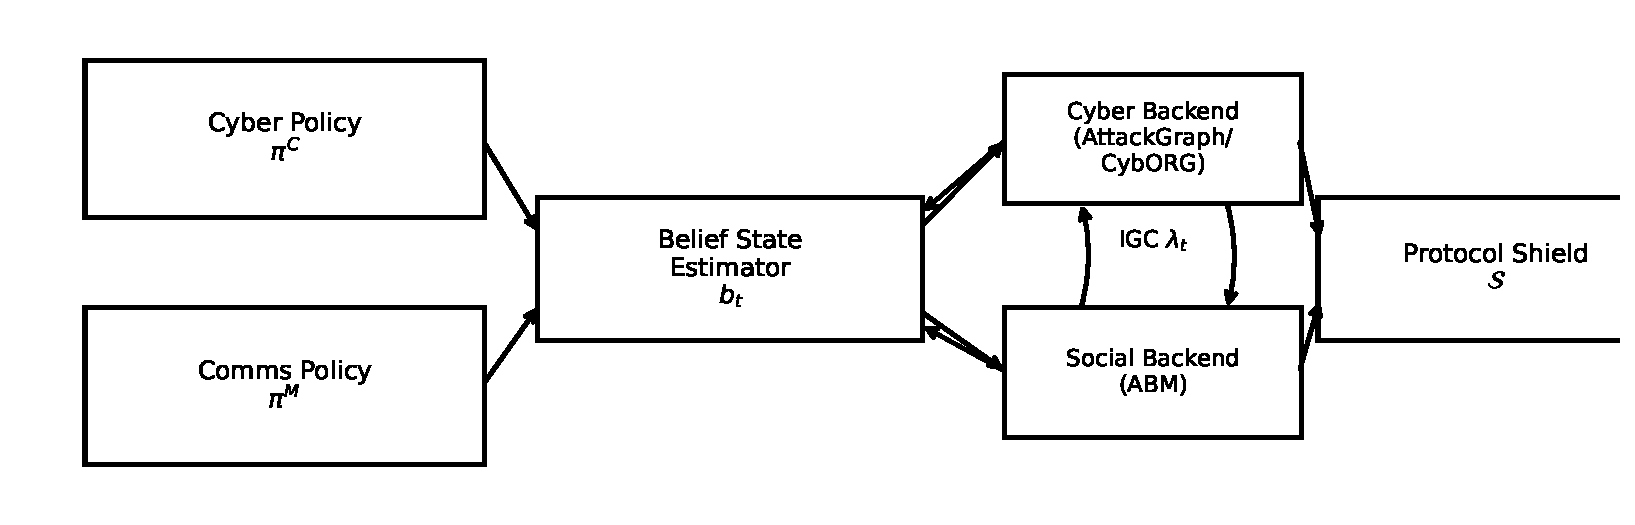
\includegraphics[width=\linewidth]{figures/fig_architecture_igc.pdf}
\caption{\model{} architecture with \igc{}. Two cooperating agents select cyber operations and crisis communications. Immune-gated coupling computes an activation variable $\lambda_t$ from a cyber danger proxy and social uncertainty; $\lambda_t$ gates when social-to-cyber feedback (compliance and reporting modifiers) is trusted and incorporated into cyber decision-making. In parallel, antigen-driven memory scales messaging intensity and targeting. Communication actions are filtered by a runtime protocol shield that guarantees zero executed protocol violations while logging attempted violations and interventions for auditability.}
\label{fig:arch}
\end{figure*}


\subsection{Cyber policy}
The cyber policy $\pi^C(a^C_t \mid o^C_t, b_t)$ selects operational actions. In this work we instantiate $\pi^C$ using a rule-based incident-response controller with configurable aggressiveness and prioritization (patch versus isolate versus restore). This provides a transparent baseline suitable for ablation and reproducibility; the framework is compatible with learned policies (e.g., MARL) in future work.

\subsection{Communication policy with targeting}
The communication policy $\pi^M(a^M_t \mid o^S_t, b_t)$ proposes messaging actions conditioned on the estimated sentiment state. We distinguish targeted messaging, which focuses interventions on communities with high misbelief or low trust, from non-targeted broadcast messaging. Targeting is implemented via a community-level risk estimator that ranks subpopulations by misinformation exposure and susceptibility.

\subsection{Coupling function}
A coupling function $\Phi$ maps social macro-state to cyber-relevant quantities. In \envname{}, compliance affects the effectiveness of operational mitigation (e.g., patch adoption and isolation adherence) and reporting affects detection probability (e.g., user-reported phishing). Trust moderates how strongly official messages shift beliefs. Conversely, cyber events (service loss, confirmed compromise) inject narrative shocks that perturb social dynamics, capturing how technical realities shape online discourse.


\subsection{Immune-gated coupling (IGC): danger, tolerance, and escalation}
\label{sec:igc}
Naive coupling can be brittle: in early incident stages, social signals may be sparse, noisy, or adversarially manipulated, yet an aggressively coupled controller may overreact (e.g., amplifying operational disruptions or issuing premature corrections).
To make coupling more robust, we introduce \emph{immune-gated coupling} (IGC), inspired by danger theory and immune tolerance \citep{matzinger1994tolerance}.
IGC regulates \emph{when} the controller relies on cyber--social feedback and \emph{how strongly} it targets and intensifies counter-messaging.

\paragraph{Cyber ``danger'' signal.}
Let $\mathrm{sev}_t \in [0,1]$ denote a normalized incident severity proxy (e.g., service loss and compromise indicators), and let $\mathrm{conf}_t \in [0,1]$ denote detection confidence.
We compute a scalar danger score
\begin{equation}
d_t = \mathrm{clip}\big(w_{\mathrm{sev}}\cdot \mathrm{sev}_t + w_{\mathrm{gap}}\cdot \max(0, \theta_{\mathrm{det}} - \mathrm{conf}_t),\, 0,\, 1\big),
\end{equation}
where $\theta_{\mathrm{det}}$ is a ``good enough'' confidence reference and $\mathrm{clip}$ truncates to $[0,1]$.

\paragraph{Coupling activation under uncertainty.}
We gate coupling based on credible danger and sufficiently informative social measurements.
Let $\mathrm{unc}_t \in [0,1]$ denote aggregate social uncertainty.
The IGC activation variable is
\begin{equation}
\lambda_t = \mathbb{I}\!\left[d_t \ge \tau_d \;\wedge\; \mathrm{unc}_t \le \tau_u\right].
\end{equation}
When $\lambda_t = 0$, the cyber controller falls back to a conservative decoupled response (akin to a ``tolerant'' immune state); when $\lambda_t = 1$, social-to-cyber modifiers (compliance and reporting) are trusted and incorporated into cyber action selection.

\paragraph{Community ``antigen'' score and memory.}
For each community $c$, we define an antigen score from the social macro-state:
\begin{equation}
a_{c,t} = w_M \cdot \mathrm{misbelief}_{c,t} \;+\; w_T \cdot (1-\mathrm{trust}_{c,t}) \;+\; w_U \cdot \mathrm{uncertainty}_{c,t} \;+\; w_P \cdot \mathrm{polarization}_{c,t}.
\end{equation}
IGC maintains an exponential moving average (immune ``memory'')
\begin{equation}
m_{c,t} = (1-\rho)\,m_{c,t-1} + \rho\,a_{c,t},
\end{equation}
which stabilizes targeting against transient noise.

\paragraph{Targeting, ``clonal expansion'', and systemic triggers.}
Communities with $m_{c,t} \ge \tau_a$ are eligible for targeted corrections, and the top-$K$ highest-risk communities are selected when targeted messaging is enabled.
Message intensity is scaled via
\begin{equation}
I_t = \mathrm{clip}\!\left(I_0 + \kappa \cdot \max_c m_{c,t},\, I_{\min},\, I_{\max}\right),
\end{equation}
capturing a clonal-expansion analogy: higher antigen load elicits stronger response.
Finally, when the fraction of communities above $\tau_a$ exceeds a threshold $\phi$, IGC triggers a systemic broadcast mode (respond broadly rather than narrowly).

\paragraph{Immune checkpoints via protocol enforcement.}
All communication actions proposed under IGC (or any controller) are filtered by the runtime protocol shield (Section~\ref{sec:protocol}), which functions analogously to an immune checkpoint by preventing ``autoimmune'' unsafe statements from executing while preserving an auditable intervention log.

\begin{table}[t]
\centering
\caption{Mapping from immune mechanisms to V-CHIMERA+IGC components.}
\label{tab:immune_mapping}
\small
\setlength{\tabcolsep}{4pt}
\begin{tabular}{p{0.34\linewidth}p{0.60\linewidth}}
\toprule
Immune mechanism & Realization in V-CHIMERA+IGC \\
\midrule
Danger signaling \citep{matzinger1994tolerance} & Cyber danger score $d_t$ from severity and detection-confidence gap. \\
Antigen recognition & Community antigen score $a_{c,t}$ combining misbelief, trust risk, uncertainty, and polarization. \\
Immune memory & Exponential smoothing $m_{c,t}$ for stable community risk ranking. \\
Tolerance / activation thresholds & Coupling activation $\lambda_t$ requires $d_t\ge\tau_d$ and $\mathrm{unc}_t\le\tau_u$; targeting requires $m_{c,t}\ge\tau_a$. \\
Clonal expansion & Messaging intensity $I_t$ increases with $\max_c m_{c,t}$; top-$K$ communities are prioritized. \\
Systemic response & Broadcast trigger when a large fraction of communities exceed $\tau_a$. \\
Immune checkpoints & Protocol shield prevents unsafe communications and logs edits. \\
\bottomrule
\end{tabular}
\end{table}

\begin{algorithm}[t]
\caption{Immune-gated coupling regulator (IGC) at time $t$}
\label{alg:igc}
\begin{algorithmic}[1]
\Require Cyber proxies $(\mathrm{sev}_t,\mathrm{conf}_t)$, social uncertainty $\mathrm{unc}_t$, community metrics $\{\mathrm{misbelief}_{c,t},\mathrm{trust}_{c,t},\mathrm{uncertainty}_{c,t},\mathrm{polarization}_{c,t}\}_c$, memory $\{m_{c,t-1}\}_c$
\Ensure Coupling activation $\lambda_t$, target set $\mathcal{C}_t$, intensity $I_t$, updated memory $\{m_{c,t}\}_c$
\State $d_t \leftarrow \mathrm{clip}(w_{\mathrm{sev}}\mathrm{sev}_t + w_{\mathrm{gap}}\max(0,\theta_{\mathrm{det}}-\mathrm{conf}_t),0,1)$
\State $\lambda_t \leftarrow \mathbb{I}[d_t \ge \tau_d \wedge \mathrm{unc}_t \le \tau_u]$
\For{each community $c$}
  \State $a_{c,t} \leftarrow w_M\mathrm{misbelief}_{c,t} + w_T(1-\mathrm{trust}_{c,t}) + w_U\mathrm{uncertainty}_{c,t} + w_P\mathrm{polarization}_{c,t}$
  \State $m_{c,t} \leftarrow (1-\rho)m_{c,t-1} + \rho a_{c,t}$
\EndFor
\State $\mathcal{C}_t \leftarrow \textsc{TopK}\big(\{c : m_{c,t}\ge\tau_a\}\big)$
\If{$\frac{|\{c: m_{c,t}\ge\tau_a\}|}{|\mathcal{C}|} \ge \phi$}
  \State $\mathcal{C}_t \leftarrow \mathcal{C}$ \Comment{systemic broadcast}
\EndIf
\State $I_t \leftarrow \mathrm{clip}(I_0 + \kappa\max_c m_{c,t}, I_{\min}, I_{\max})$
\end{algorithmic}
\end{algorithm}


\section{Communication protocol and runtime shield}
A central design principle in \model{} is that crisis communications are safety-critical actions. Unlike many cyber actions, harmful public statements can cause irreversible damage. We therefore represent communication governance as a protocol and enforce it at runtime.

\subsection{Protocol as constraint predicates}
Let $a^M_t$ be a communication action parameterized by an intent (e.g., status update, rumor correction), targeting scope (broadcast versus communities), and certainty level. We define safety predicates $\{g_k\}_{k=1}^K$ such that a message is safe iff
\begin{equation}
\forall k,\quad g_k(s_t, a^M_t) \le 0.
\end{equation}
In the artifact, $g_k$ is implemented as a lightweight rule set checking for over-claiming (high certainty with low detection confidence), over-disclosure (naming specific assets or unverified root causes), harmful instructions, and contradictions with earlier official statements.

\subsection{Shield operation}
Given a proposed action $a^M_t$ from the comms policy, the shield computes
\begin{equation}
\tilde a^M_t = \mathcal{S}(a^M_t, s_t),
\end{equation}
where $\tilde a^M_t = a^M_t$ if safe; otherwise $\tilde a^M_t$ is the nearest safe alternative under a discrete edit distance (e.g., downgrade certainty, switch to a hold statement, or remove targeting). This follows the ``optimize under soft objectives, enforce hard constraints at runtime'' principle \citep{alshiekh2018safe,koenighofer2024shields}.

\subsection{End-to-end step algorithm}
Algorithm~\ref{alg:step} summarizes the closed-loop interaction.

\begin{algorithm}[t]
\caption{\model{} closed-loop step (single episode)}
\label{alg:step}
\begin{algorithmic}[1]
\State Initialize environment state $s_0$, observations $o_0$, and belief state $b_0$
\For{$t=0,\dots,T-1$}
  \State Observe $(o^C_t, o^S_t)$
  \State Update belief $b_t \leftarrow \textsc{Estimate}(b_{t-1}, o_t)$
  \State Propose cyber action $a^C_t \sim \pi^C(\cdot \mid o^C_t, b_t)$
  \State Propose comms action $a^M_t \sim \pi^M(\cdot \mid o^S_t, b_t)$
  \State Enforce protocol $\tilde a^M_t \leftarrow \mathcal{S}(a^M_t, s_t)$
  \State Step environment $(s_{t+1}, o_{t+1}) \leftarrow \mathcal{P}(s_t, a^C_t, \tilde a^M_t)$
  \State Log metrics (harm, misbelief, trust, violations, edits)
\EndFor
\end{algorithmic}
\end{algorithm}

\section{\envname{} coupled cyber--social testbed}
\envname{} couples (i) a cyber incident simulator and (ii) a multi-platform social-network agent-based model, enabling closed-loop evaluation.

\subsection{Cyber backend}
The default cyber backend is an attack-graph simulator with stochastic attacker progression and defender actions under resource constraints. The defender can isolate nodes, patch vulnerabilities, restore services, and allocate detection effort. Cyber harm aggregates availability loss, compromise spread, and exfiltration proxies. While simplified relative to a real enterprise network, the backend supports heterogeneous assets, multiple attacker objectives, and action costs, enabling systematic ablations.

\subsection{Social backend}
The social backend simulates a population partitioned into communities and exposed to multiple platforms. Individuals update beliefs based on peer exposure, bot-driven misinformation injection, official communication, and platform moderation (removal and labeling). The model outputs macro metrics---misbelief, trust, uncertainty, and polarization---which define the sentiment state coupled to cyber dynamics.

\subsection{Calibration}
Agent-based models can exhibit degenerate regimes (immediate consensus or total fragmentation). We therefore include a calibration routine that searches parameter space to match stylized crisis-regime target intervals. 

\section{Experimental Methodology}
\label{sec:method}

\subsection{Scenarios}
We evaluate three cyber--social crisis scenarios: \textit{ransomware rumor}, \textit{service outage rumor}, and \textit{exfiltration scam}.
Each scenario specifies (i) a distribution over cyber incident traces, (ii) an initial narrative shock, and (iii) an adversarial misinformation or scam strategy (bot injection and opportunistic fraud) operating under platform moderation.

\subsection{Policies}
We compare sequential and coupled incident-response controllers, with and without runtime protocol enforcement:
\begin{itemize}[leftmargin=*]
  \item \textbf{Pipeline}: sequential baseline (cyber response + generic communication), no coupling and no shield.
  \item \textbf{Pipeline+Shield}: baseline pipeline with protocol enforcement enabled.
  \item \textbf{V-CHIMERA}: coupled cyber+communication controller without a shield.
  \item \textbf{V-CHIMERA+Shield}: naive coupling with protocol enforcement.
  \item \textbf{V-CHIMERA+IGC+Shield}: immune-gated coupling (IGC) with protocol enforcement. This biomimetic variant regulates when the cyber controller \emph{relies on social feedback} by requiring a high cyber ``danger'' signal and sufficiently low social uncertainty; in parallel, community-level ``antigen'' scores drive targeted messaging intensity and a systemic broadcast trigger. The goal is to avoid overreaction to noisy sentiment signals while still escalating under credible threat.
  \item \textbf{No coupling+Shield}: ablation that disables cyber--social coupling while keeping shielding.
  \item \textbf{No targeting+Shield}: ablation that disables community targeting (broadcast-only) while keeping shielding.
\end{itemize}

\subsection{Metrics and reporting}
We report time-normalized area-under-curve (AUC) metrics over the episode horizon: cyber harm (lower is better), misbelief (lower is better), trust (higher is better), uncertainty (lower is better), and polarization (lower is better).
Protocol safety is measured by attempted violations, executed violations, and the number of shield edits.
Each scenario--policy pair is evaluated over eight random seeds; we report mean $\pm$ one standard deviation over seeds (SD). Where useful, paired permutation tests are reported to quantify the robustness of differences across seeds.

\section{Results}
\label{sec:results}

Table~\ref{tab:main} reports aggregate cyber and social outcomes across scenarios, while Table~\ref{tab:protocol} summarizes protocol compliance. Figures~\ref{fig:tradeoff}--\ref{fig:sensitivity} visualize trade-offs and macro-dynamics.

\begin{table*}[t]
\centering
\caption{Main results (mean $\pm$ SD over seeds). Lower is better for cyber harm and misbelief; higher is better for trust. ``Exec. viol.'' counts executed protocol violations (0 for all shielded policies). ``Shield edits'' counts runtime interventions by the communication shield. Boldface indicates the best shielded result per scenario for each primary metric.}
\label{tab:main}
\small
\setlength{\tabcolsep}{3pt}
\resizebox{\linewidth}{!}{\begin{tabular}{llccccc}
\toprule
Scenario & Policy & Cyber harm AUC $\downarrow$ & Misbelief AUC $\downarrow$ & Trust AUC $\uparrow$ & Exec. viol. $\downarrow$ & Shield edits $\downarrow$ \\
\midrule
\multirow{7}{*}{Exfiltration scam} & Pipeline & 2.648 $\pm$ 0.601 & 0.688 $\pm$ 0.119 & 0.134 $\pm$ 0.086 & 162.750 $\pm$ 38.936 & 0.000 $\pm$ 0.000 \\
 & Pipeline+Shield & 2.554 $\pm$ 0.532 & 0.771 $\pm$ 0.129 & 0.137 $\pm$ 0.086 & 0.000 $\pm$ 0.000 & 47.625 $\pm$ 10.600 \\
 & V-CHIMERA & 2.454 $\pm$ 0.676 & 0.694 $\pm$ 0.176 & 0.238 $\pm$ 0.121 & 48.625 $\pm$ 12.642 & 0.000 $\pm$ 0.000 \\
 & V-CHIMERA+Shield & 2.616 $\pm$ 0.522 & 0.750 $\pm$ 0.130 & 0.166 $\pm$ 0.099 & 0.000 $\pm$ 0.000 & 35.500 $\pm$ 5.568 \\
 & V-CHIMERA+IGC+Shield & 2.502 $\pm$ 0.716 & 0.739 $\pm$ 0.157 & 0.155 $\pm$ 0.120 & 0.000 $\pm$ 0.000 & 35.000 $\pm$ 9.429 \\
 & No coupling+Shield & 2.495 $\pm$ 0.708 & 0.739 $\pm$ 0.156 & 0.165 $\pm$ 0.113 & 0.000 $\pm$ 0.000 & 32.500 $\pm$ 8.851 \\
 & No targeting+Shield & \textbf{2.482 $\pm$ 0.703} & \textbf{0.676 $\pm$ 0.181} & \textbf{0.194 $\pm$ 0.137} & 0.000 $\pm$ 0.000 & 33.125 $\pm$ 8.531 \\
\midrule
\multirow{7}{*}{Outage rumor} & Pipeline & 0.819 $\pm$ 0.739 & 0.365 $\pm$ 0.151 & 0.398 $\pm$ 0.144 & 56.250 $\pm$ 54.262 & 0.000 $\pm$ 0.000 \\
 & Pipeline+Shield & 0.791 $\pm$ 0.704 & 0.422 $\pm$ 0.189 & 0.388 $\pm$ 0.153 & 0.000 $\pm$ 0.000 & 19.750 $\pm$ 18.890 \\
 & V-CHIMERA & 1.251 $\pm$ 0.689 & 0.384 $\pm$ 0.131 & 0.462 $\pm$ 0.115 & 35.500 $\pm$ 16.378 & 0.000 $\pm$ 0.000 \\
 & V-CHIMERA+Shield & 1.307 $\pm$ 0.731 & 0.474 $\pm$ 0.178 & 0.361 $\pm$ 0.171 & 0.000 $\pm$ 0.000 & 25.750 $\pm$ 11.529 \\
 & V-CHIMERA+IGC+Shield & \textbf{0.751 $\pm$ 0.639} & 0.413 $\pm$ 0.193 & \textbf{0.392 $\pm$ 0.167} & 0.000 $\pm$ 0.000 & 17.625 $\pm$ 12.842 \\
 & No coupling+Shield & 0.753 $\pm$ 0.641 & 0.418 $\pm$ 0.188 & 0.388 $\pm$ 0.156 & 0.000 $\pm$ 0.000 & 15.875 $\pm$ 11.359 \\
 & No targeting+Shield & 1.470 $\pm$ 0.647 & \textbf{0.357 $\pm$ 0.121} & 0.316 $\pm$ 0.146 & 0.000 $\pm$ 0.000 & 24.375 $\pm$ 8.615 \\
\midrule
\multirow{7}{*}{Ransomware rumor} & Pipeline & 0.829 $\pm$ 0.742 & 0.334 $\pm$ 0.117 & 0.416 $\pm$ 0.127 & 45.375 $\pm$ 47.347 & 0.000 $\pm$ 0.000 \\
 & Pipeline+Shield & 0.829 $\pm$ 0.742 & 0.388 $\pm$ 0.163 & 0.415 $\pm$ 0.130 & 0.000 $\pm$ 0.000 & 15.625 $\pm$ 15.706 \\
 & V-CHIMERA & 1.636 $\pm$ 0.760 & 0.434 $\pm$ 0.125 & 0.423 $\pm$ 0.100 & 37.750 $\pm$ 13.848 & 0.000 $\pm$ 0.000 \\
 & V-CHIMERA+Shield & 1.463 $\pm$ 0.744 & 0.473 $\pm$ 0.177 & 0.369 $\pm$ 0.156 & 0.000 $\pm$ 0.000 & 25.750 $\pm$ 11.723 \\
 & V-CHIMERA+IGC+Shield & \textbf{0.620 $\pm$ 0.664} & \textbf{0.318 $\pm$ 0.142} & \textbf{0.470 $\pm$ 0.120} & 0.000 $\pm$ 0.000 & 11.750 $\pm$ 9.206 \\
 & No coupling+Shield & 0.622 $\pm$ 0.667 & 0.320 $\pm$ 0.140 & 0.460 $\pm$ 0.113 & 0.000 $\pm$ 0.000 & 9.625 $\pm$ 7.874 \\
 & No targeting+Shield & 1.916 $\pm$ 0.983 & 0.411 $\pm$ 0.154 & 0.332 $\pm$ 0.141 & 0.000 $\pm$ 0.000 & 22.875 $\pm$ 8.017 \\
\bottomrule
\end{tabular}
}
\end{table*}

Across scenarios, the communication shield provides a hard safety guarantee: all shielded policies execute zero protocol violations while producing an auditable log of attempted violations and edits (Table~\ref{tab:protocol}). Unshielded policies, by contrast, execute frequent violations, illustrating why crisis communication should be treated as a safety-critical control surface.

On effectiveness, the results distinguish between \emph{naive} coupling and \emph{regulated} coupling. The naive coupled controller (\texttt{vchimera+shield}) is brittle and often degrades outcomes relative to the shielded sequential baseline (\texttt{pipeline+shield}). The immune-gated coupling variant (\texttt{vchimera-ais+shield}; V-CHIMERA+IGC+Shield) mitigates this failure mode via \emph{evidence-gated escalation}: coupling is activated only when a cyber ``danger'' signal is high \emph{and} social uncertainty is not overwhelming, while ``antigen'' scores (misbelief and trust risk) determine whether responses remain broad or are intensified and targeted. In the \texttt{ransomware\_rumor} scenario, V-CHIMERA+IGC+Shield reduces cyber-harm AUC by about 25\% and misbelief AUC by about 18\% relative to Pipeline+Shield, while increasing trust by about 13\%. In \texttt{outage\_rumor} and \texttt{exfiltration\_scam}, the same immune-gated controller yields consistent (though smaller) reductions in harm and misbelief relative to Pipeline+Shield, while preserving or improving trust. Finally, the no-targeting ablation attains the strongest performance in \texttt{exfiltration\_scam}, suggesting that broad counter-messaging can outperform naive targeting when diffusion rapidly crosses community boundaries.

\subsection{Protocol compliance}
\label{sec:protocol}

\begin{table*}[t]
\centering
\caption{Protocol compliance (mean $\pm$ SD over seeds). The shield prevents unsafe communication actions from executing while logging attempted violations and edits.}
\label{tab:protocol}
\small
\setlength{\tabcolsep}{3pt}
\resizebox{\linewidth}{!}{\begin{tabular}{llccc}
\toprule
Scenario & Policy & Attempted viol. $\downarrow$ & Executed viol. $\downarrow$ & Shield edits $\downarrow$ \\
\midrule
\multirow{7}{*}{Exfiltration scam} & Pipeline & 162.750 $\pm$ 38.936 & 162.750 $\pm$ 38.936 & 0.000 $\pm$ 0.000 \\
 & Pipeline+Shield & 146.125 $\pm$ 35.045 & 0.000 $\pm$ 0.000 & 47.625 $\pm$ 10.600 \\
 & V-CHIMERA & 48.625 $\pm$ 12.642 & 48.625 $\pm$ 12.642 & 0.000 $\pm$ 0.000 \\
 & V-CHIMERA+Shield & 35.500 $\pm$ 5.568 & 0.000 $\pm$ 0.000 & 35.500 $\pm$ 5.568 \\
 & V-CHIMERA+IGC+Shield & 37.750 $\pm$ 12.776 & 0.000 $\pm$ 0.000 & 35.000 $\pm$ 9.429 \\
 & No coupling+Shield & 32.500 $\pm$ 8.851 & 0.000 $\pm$ 0.000 & 32.500 $\pm$ 8.851 \\
 & No targeting+Shield & 33.125 $\pm$ 8.531 & 0.000 $\pm$ 0.000 & 33.125 $\pm$ 8.531 \\
\midrule
\multirow{7}{*}{Outage rumor} & Pipeline & 56.250 $\pm$ 54.262 & 56.250 $\pm$ 54.262 & 0.000 $\pm$ 0.000 \\
 & Pipeline+Shield & 46.750 $\pm$ 44.774 & 0.000 $\pm$ 0.000 & 19.750 $\pm$ 18.890 \\
 & V-CHIMERA & 35.500 $\pm$ 16.378 & 35.500 $\pm$ 16.378 & 0.000 $\pm$ 0.000 \\
 & V-CHIMERA+Shield & 25.750 $\pm$ 11.529 & 0.000 $\pm$ 0.000 & 25.750 $\pm$ 11.529 \\
 & V-CHIMERA+IGC+Shield & 17.625 $\pm$ 12.842 & 0.000 $\pm$ 0.000 & 17.625 $\pm$ 12.842 \\
 & No coupling+Shield & 15.875 $\pm$ 11.359 & 0.000 $\pm$ 0.000 & 15.875 $\pm$ 11.359 \\
 & No targeting+Shield & 24.375 $\pm$ 8.615 & 0.000 $\pm$ 0.000 & 24.375 $\pm$ 8.615 \\
\midrule
\multirow{7}{*}{Ransomware rumor} & Pipeline & 45.375 $\pm$ 47.347 & 45.375 $\pm$ 47.347 & 0.000 $\pm$ 0.000 \\
 & Pipeline+Shield & 39.875 $\pm$ 41.956 & 0.000 $\pm$ 0.000 & 15.625 $\pm$ 15.706 \\
 & V-CHIMERA & 37.750 $\pm$ 13.848 & 37.750 $\pm$ 13.848 & 0.000 $\pm$ 0.000 \\
 & V-CHIMERA+Shield & 25.750 $\pm$ 11.723 & 0.000 $\pm$ 0.000 & 25.750 $\pm$ 11.723 \\
 & V-CHIMERA+IGC+Shield & 11.750 $\pm$ 9.206 & 0.000 $\pm$ 0.000 & 11.750 $\pm$ 9.206 \\
 & No coupling+Shield & 9.625 $\pm$ 7.874 & 0.000 $\pm$ 0.000 & 9.625 $\pm$ 7.874 \\
 & No targeting+Shield & 22.875 $\pm$ 8.017 & 0.000 $\pm$ 0.000 & 22.875 $\pm$ 8.017 \\
\bottomrule
\end{tabular}
}
\end{table*}

\subsection{Cyber--social trade-offs}
To visualize cyber--social trade-offs, Figure~\ref{fig:tradeoff} plots misbelief versus cyber harm for each scenario. The accent marker highlights the immune-gated controller (\texttt{vchimera-ais+shield}).

\begin{figure}[t]
  \centering
  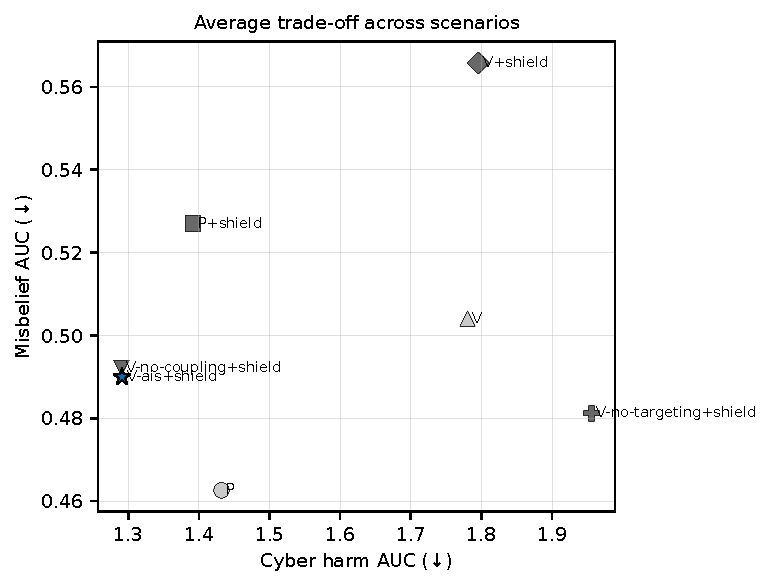
\includegraphics[width=.85\linewidth]{figures/fig_tradeoff_bw.pdf}
  \caption{Trade-offs between cyber harm and misbelief (mean across seeds). Each point corresponds to a policy. Arrows indicate the direction of improvement (lower is better for both axes); the accent marker highlights the immune-gated coupled system (\texttt{vchimera-ais+shield}).}
  \label{fig:tradeoff}
\end{figure}

\subsection{Statistical comparison of immune-gated coupling}
To complement the descriptive uncertainty in Tables~\ref{tab:main}--\ref{tab:protocol}, we run an exact paired sign-flip permutation test across seeds comparing \texttt{vchimera-ais+shield} (V-CHIMERA+IGC+Shield) to the non-biomimetic coupled controller \texttt{vchimera+shield} (V-CHIMERA+Shield).
Table~\ref{tab:permtests} reports mean paired differences $\Delta$ (IGC minus coupled) and corresponding two-sided $p$-values for the primary outcomes.
Consistent with the ``avoid autoimmune overreaction'' design goal, IGC yields significant reductions in cyber-harm AUC in the \texttt{ransomware\_rumor} and \texttt{outage\_rumor} scenarios, while sentiment improvements are more scenario-dependent.

\begin{table}[t]
\centering
\caption{Paired permutation tests comparing V-CHIMERA+IGC+Shield to V-CHIMERA+Shield across seeds ($n{=}8$). $\Delta$ denotes mean paired difference (IGC minus coupled). Lower is better for harm and misbelief; higher is better for trust.}
\label{tab:permtests}
\small
\setlength{\tabcolsep}{4pt}
\resizebox{\linewidth}{!}{\begin{tabular}{lrrrrrr}
\toprule
Scenario & $\Delta$Harm & $p$ & $\Delta$Misbelief & $p$ & $\Delta$Trust & $p$ \\
\midrule
ransomware\_rumor & -0.843 & 0.031 & -0.155 & 0.125 & +0.101 & 0.211 \\
outage\_rumor & -0.556 & 0.047 & -0.061 & 0.500 & +0.031 & 0.594 \\
exfiltration\_scam & -0.114 & 0.648 & -0.011 & 1.000 & -0.011 & 0.695 \\
\bottomrule
\end{tabular}
}
\end{table}



\subsection{Macro-dynamics over time}
Belief and trust trajectories are visualized in Figure~\ref{fig:timeseries_grid}, while Figure~\ref{fig:polarization_grid} reports uncertainty and polarization dynamics.

\begin{figure*}[t]
  \centering
  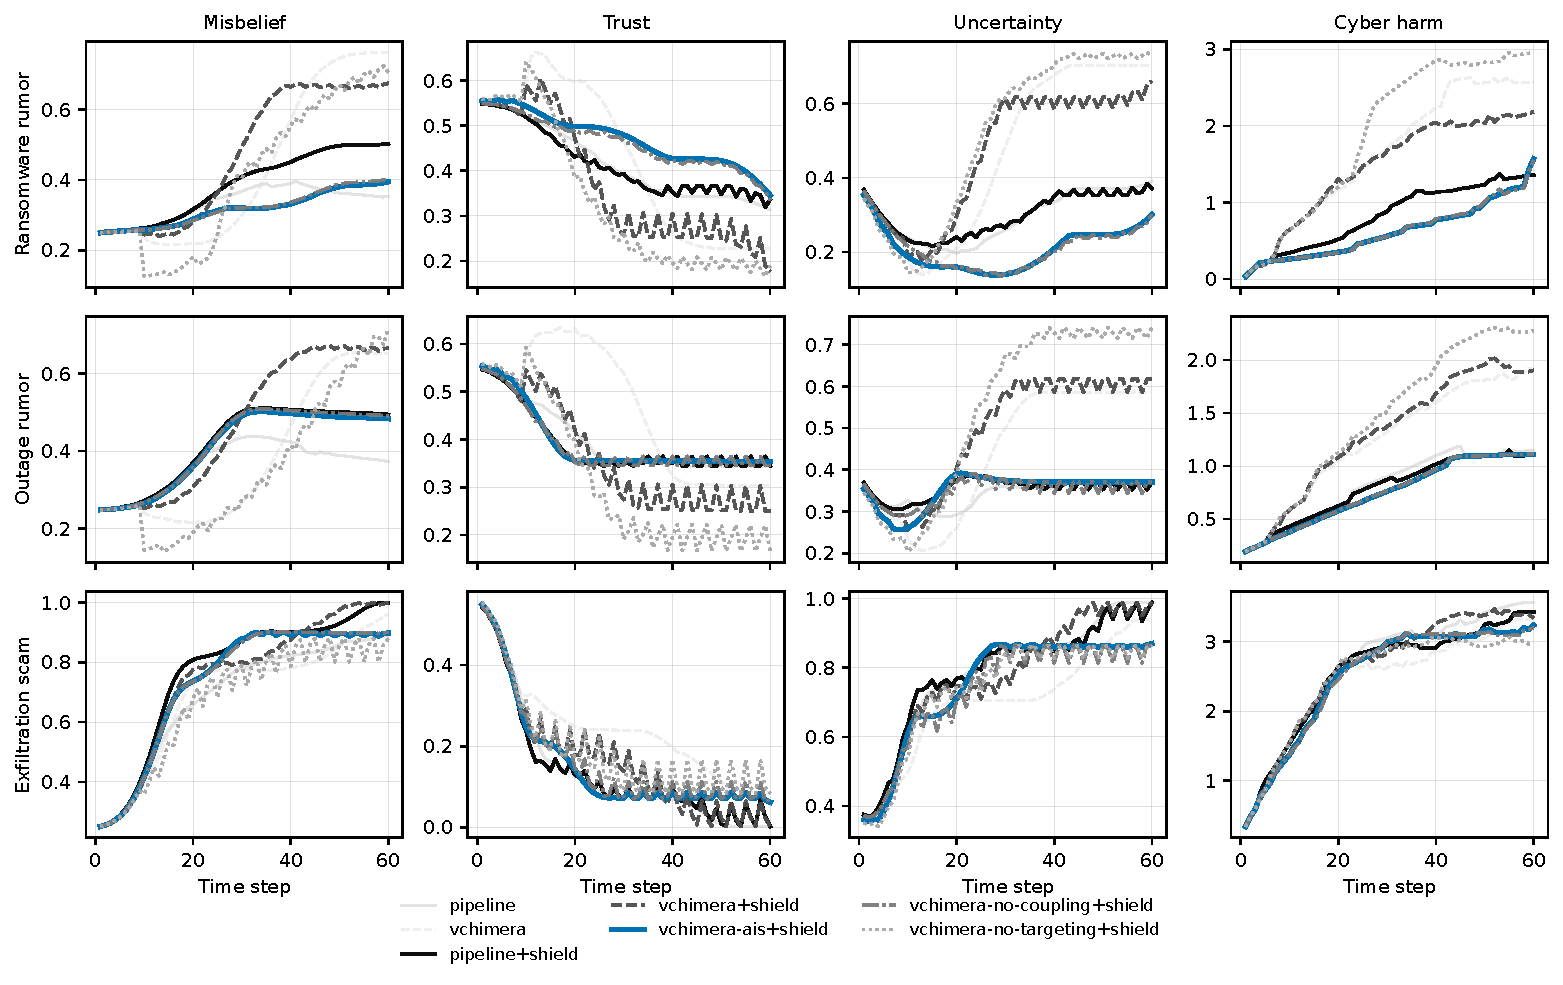
\includegraphics[width=\linewidth]{figures/fig_timeseries_grid_gray.pdf}
  \caption{Macro-dynamics over time (mean across seeds). Rows correspond to scenarios; columns show cyber harm, misbelief, and trust. The immune-gated controller (accent line) improves stability in \texttt{ransomware\_rumor} while maintaining protocol safety.}
  \label{fig:timeseries_grid}
\end{figure*}

\begin{figure*}[t]
  \centering
  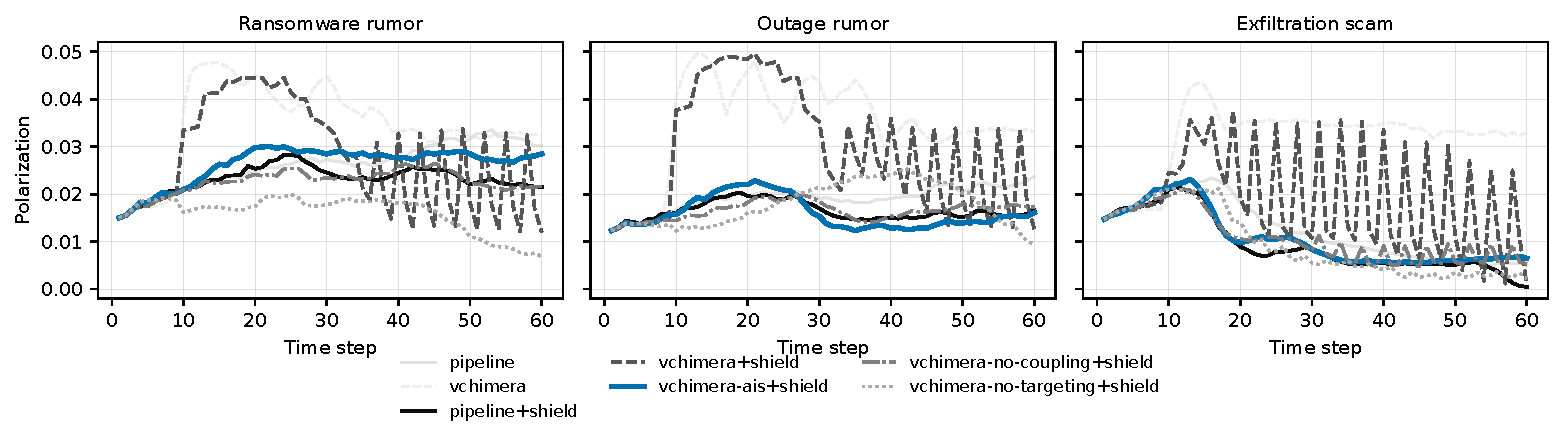
\includegraphics[width=\linewidth]{figures/fig_polarization_grid_gray.pdf}
  \caption{Uncertainty and polarization dynamics (mean across seeds). Rows correspond to scenarios; columns show uncertainty and polarization.}
  \label{fig:polarization_grid}
\end{figure*}

\subsection{Robustness and sensitivity}
\label{sec:sensitivity}
We perform a grid sensitivity analysis for the \texttt{ransomware\_rumor} scenario by varying (i) cyber--social coupling strength and (ii) platform moderation effectiveness. We evaluate both the naive coupled controller (\texttt{vchimera+shield}) and the immune-gated controller (\texttt{vchimera-ais+shield}).
Figure~\ref{fig:sensitivity} shows that naive coupling becomes brittle as coupling strengthens and moderation weakens (misbelief increases), whereas immune-gated coupling attenuates this amplification and yields consistently lower misbelief. Table~\ref{tab:sensitivity} summarizes the effect at two extreme settings.

\begin{figure}[t]
  \centering
  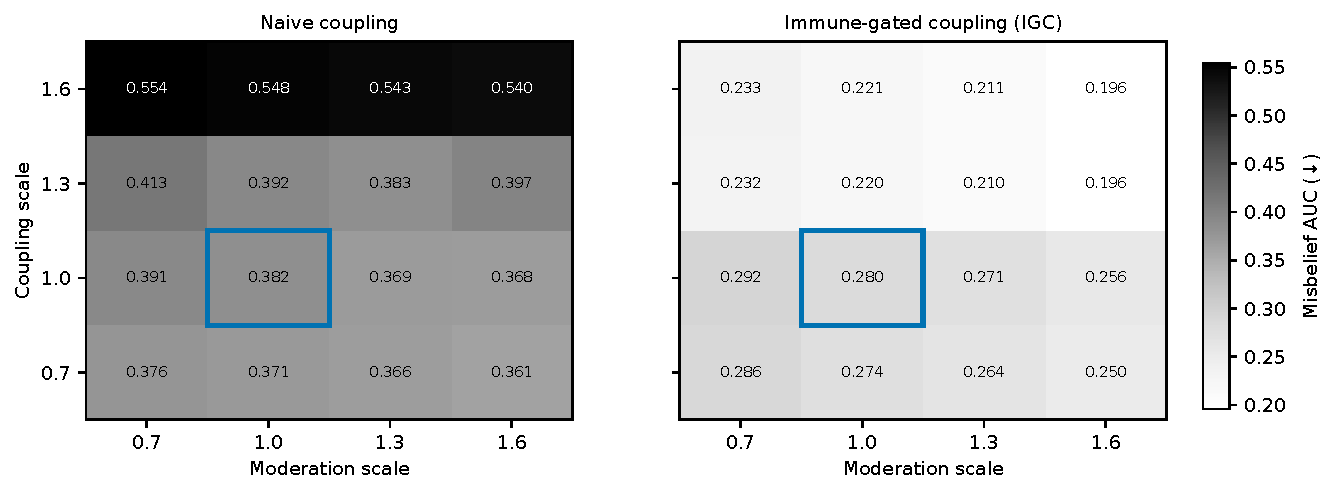
\includegraphics[width=.85\linewidth]{figures/fig_sensitivity_compare_gray.pdf}
  \caption{Sensitivity of misbelief AUC in \texttt{ransomware\_rumor} as a function of cyber--social coupling and platform moderation. Left: naive coupling (V-CHIMERA+Shield). Right: immune-gated coupling (V-CHIMERA+IGC+Shield).}
  \label{fig:sensitivity}
\end{figure}

\begin{table}[t]
\centering
\caption{Sensitivity summary at extreme settings (\texttt{ransomware\_rumor}). Values report misbelief AUC for the naive coupling controller and the immune-gated coupling (IGC) controller.}
\label{tab:sensitivity}
\small
\begin{tabular}{lccc}
\toprule
Setting & Naive coupling & Immune-gated coupling (IGC) & $\Delta$ (Naive -- IGC) \\
\midrule
Low coupling / high moderation & 0.361 & 0.250 & 0.111 \\
High coupling / low moderation & 0.554 & 0.233 & 0.321 \\
\bottomrule
\end{tabular}

\end{table}

\section{Discussion}
Our evaluation supports three qualitative conclusions relevant to socio-technical incident response.

First, coupling communication into operations can help when the cyber--social linkage is strong and correctly specified. In such regimes, the policy can trade operational actions against sentiment dynamics, improving trust and reducing misbelief with limited operational cost. However, when linkage is weak or misspecified, coupling can increase cyber harm. Practical systems should therefore (i) gate coupling on evidence of social-to-cyber impact, (ii) estimate coupling online, or (iii) fall back to a decoupled safe policy when linkage is uncertain.

Second, targeting is valuable when susceptibility is heterogeneous and attention is constrained, but it is not universally dominant. Our ablations suggest that broad counter-messaging can outperform naive targeting in regimes where diffusion rapidly crosses community boundaries or where the model lacks explicit attention/reach constraints. Treating targeting as a tunable design choice---and incorporating empirically grounded segmentation and platform recommender effects---is a key direction for future work.

Third, protocol enforcement is necessary for deployment. Even if an unconstrained policy improves average performance, rare but severe communication failures are unacceptable. The shield provides a clean separation: optimize under soft objectives and enforce hard constraints at runtime, yielding both safety guarantees and auditable intervention logs.

\section{Implications}
For security operations centers and organizational communications units, the results motivate treating crisis communication as an operational control surface rather than an afterthought. Maintaining an explicit sentiment-state estimate (misbelief, trust, uncertainty) enables allocating messaging resources to communities at highest misinformation risk. The protocol shield provides a governance mechanism: organizations can encode policy constraints (e.g., ``do not debunk without evidence'' or ``label uncertainty when uncertainty is high'') and guarantee compliance even when a learned policy proposes unsafe actions. Shield-edit counts and violation logs provide auditable signals for after-action review and continuous improvement of incident playbooks.

At a societal level, verified, evidence-grounded crisis communication can reduce exposure to follow-on scams and avoid overconfident corrections that undermine trust. More broadly, this work illustrates how socio-technical safety mechanisms can be embedded into automated decision systems to protect public trust during disruptive events.

\section{Limitations}
Our study has limitations that motivate future work. The default cyber backend is an abstract incident simulator and omits real-network complexities (legacy constraints, hidden dependencies, and incomplete telemetry). The social ABM is stylized and does not model full language semantics or platform recommender systems. We partially address external validity by exposing parameters, providing calibration tools, and including an adapter scaffold for CybORG, but richer backends and empirical grounding are needed for deployment.

Our baseline policies are intentionally transparent and reproducible. Incorporating learned policies (e.g., MARL) with the same shield may yield stronger performance while retaining guarantees. Finally, trust and belief are represented by proxy variables; real-world use requires careful empirical validation and ethical oversight.

\section{Conclusion}
We introduced \model{}, a misinformation-aware incident response framework that couples cyber operations and crisis communication under explicit protocol constraints.
The communication shield enforces a hard safety guarantee (zero executed protocol violations) while producing an auditable record of attempted violations and runtime edits.
Empirically, our results highlight a key biomimetic insight: \emph{naive} coupling can be brittle and may amplify misinformation-driven disruption, but an \emph{immune-gated coupling} (IGC) controller---inspired by immune tolerance and danger signaling---mitigates this failure mode by escalating coupling and messaging only when evidence warrants it.
Across our scenarios, the immune-gated controller improves the cyber--social trade-off relative to shielded sequential baselines, and sensitivity analysis shows that IGC attenuates the degradation observed under strong coupling and weak moderation.
We hope this work stimulates cybersecurity research on closed-loop cyber--social crises and biomimetic control design for verified socio-technical decision systems that align operational effectiveness with governance constraints.

%%%%%%%%%%%%%%%%%%%%%%%%%%%%%%%%%%%%%%%%%%
\vspace{6pt} 

%%%%%%%%%%%%%%%%%%%%%%%%%%%%%%%%%%%%%%%%%%
%% optional
%\supplementary{The following supporting information can be downloaded at:  \linksupplementary{s1}, Figure S1: title; Table S1: title; Video S1: title.}

% Only for journal Methods and Protocols:
% If you wish to submit a video article, please do so with any other supplementary material.
% \supplementary{The following supporting information can be downloaded at: \linksupplementary{s1}, Figure S1: title; Table S1: title; Video S1: title. A supporting video article is available at doi: link.}

% Only used for preprtints:
% \supplementary{The following supporting information can be downloaded at the website of this paper posted on \href{https://www.preprints.org/}{Preprints.org}.}

% Only for journal Hardware:
% If you wish to submit a video article, please do so with any other supplementary material.
% \supplementary{The following supporting information can be downloaded at: \linksupplementary{s1}, Figure S1: title; Table S1: title; Video S1: title.\vspace{6pt}\\
%\begin{tabularx}{\textwidth}{lll}
%\toprule
%\textbf{Name} & \textbf{Type} & \textbf{Description} \\
%\midrule
%S1 & Python script (.py) & Script of python source code used in XX \\
%S2 & Text (.txt) & Script of modelling code used to make Figure X \\
%S3 & Text (.txt) & Raw data from experiment X \\
%S4 & Video (.mp4) & Video demonstrating the hardware in use \\
%... & ... & ... \\
%\bottomrule
%\end{tabularx}
%}

%%%%%%%%%%%%%%%%%%%%%%%%%%%%%%%%%%%%%%%%%%
%%%%%%%%%%%%%%%%%%%%%%%%%%%%%%%%%%%%%%%%%%
\authorcontributions{Conceptualization, F.A. and S.A.; methodology, F.A. and S.A.; software, F.A. and S.A.; validation, F.A. and S.A.; formal analysis, F.A. and S.A.; investigation, F.A. and S.A.; resources, S.A.; data curation, F.A. and S.A.; writing---original draft preparation, F.A.; writing---review and editing, F.A. and S.A.; visualization, F.A. and S.A.; supervision, S.A.; project administration, S.A.; funding acquisition, S.A. All authors have read and agreed to the published version of the manuscript.}

\funding{This research received no external funding.}% The APC was funded by the author.}

\institutionalreview{Not applicable.}

\informedconsent{Not applicable.}

\dataavailability{The simulation code, configuration files, and figure-generation scripts used in this study are included in the supplementary submission package (anonymized for review). The results reported in the manuscript can be reproduced by running the provided pipeline; all data are generated via simulation.}

\acknowledgments{The authors thank the open-source community for software tools that supported this work.}

% Optional (only if required by the journal):
% \useofartificialintelligence{During the preparation of this manuscript, the author used ChatGPT (OpenAI) for language editing and LaTeX formatting support. The author reviewed and edited the output and takes full responsibility for the content.}

\conflictsofinterest{The authors declare no conflicts of interest.}


%%%%%%%%%%%%%%%%%%%%%%%%%%%%%%%%%%%%%%%%%%
%% Optional

%% Only for journal Encyclopedia
%\entrylink{The Link to this entry published on the encyclopedia platform.}

\abbreviations{Abbreviations}{
The following abbreviations are used in this manuscript:
\\

\noindent
\begin{tabular}{@{}ll}
ABM & Agent-based model\\
AUC & Area under the curve\\
IGC & Immune-gated coupling\\
IR & Incident response\\
MAS & Multi-agent system\\
POMDP & Partially observable Markov decision process\\
POSG & Partially observable stochastic game\\
SOC & Security operations center\\
V-CHIMERA & Verified coupled human--information--machine incident response architecture\\
\end{tabular}
}

%%%%%%%%%%%%%%%%%%%%%%%%%%%%%%%%%%%%%%%%%%
%% Optional
\appendixtitles{no} % Leave argument "no" if all appendix headings stay EMPTY (then no dot is printed after "Appendix A"). If the appendix sections contain a heading then change the argument to "yes".
\appendixstart
\appendix


\section{Additional dynamics: polarization}
\label{app:polarization}
Polarization trajectories provide a complementary view of social stability beyond misbelief and trust. Figure~\ref{fig:pol_grid} reports polarization over time across the three primary scenarios and the illustrative CybORG transfer run.

\begin{figure}[t]
  \centering
  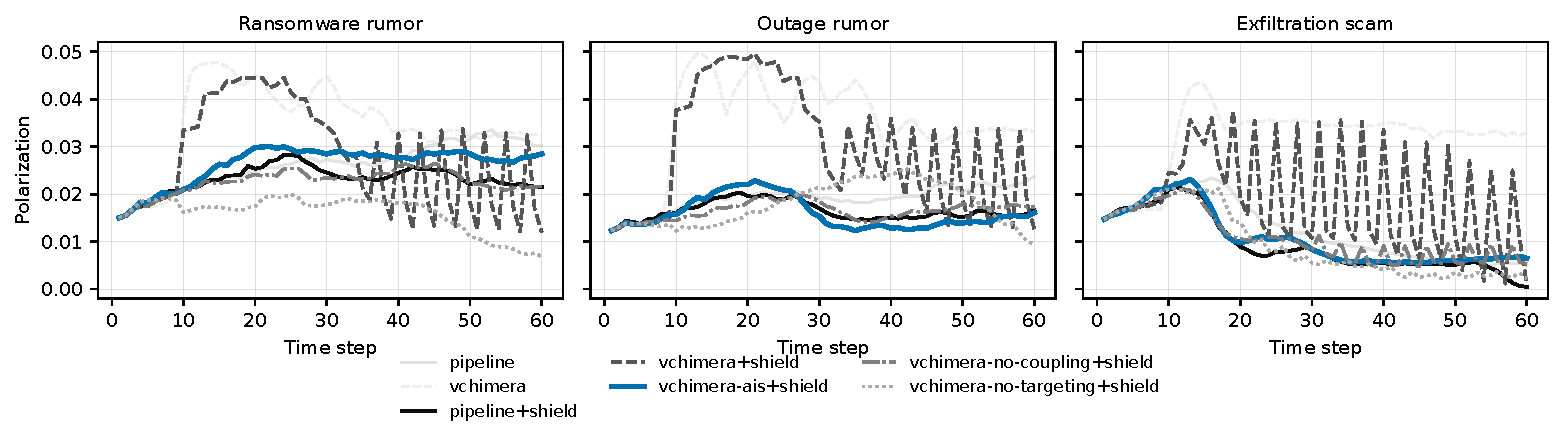
\includegraphics[width=\linewidth]{figures/fig_polarization_grid_gray.pdf}
  \caption{Polarization over time (mean across seeds). Panels correspond to ransomware rumor, outage rumor, exfiltration scam, and the illustrative CybORG transfer run.}
  \label{fig:pol_grid}
\end{figure}

\section{CybORG transfer experiment (artifact extension)}
\label{app:cyborg}
To demonstrate extensibility beyond the default incident backend, the artifact includes an adapter for the CybORG ecosystem \citep{baillie2020cyborg,standen2021cyborg,emerson2024cyborgpp}. CybORG provides a higher-fidelity enterprise-defense setting with richer cyber observations than an abstract attack-graph simulator.

\subsection{Adapter mapping}
The adapter maps CybORG observations (e.g., service availability, detection signals, evidence proxies) into the shared cyber state used by the coupling bus and protocol monitor, enabling the same communication shield and sentiment dynamics to be exercised in the CybORG loop.

\subsection{Illustrative transfer run}
We include an illustrative run on the CC4 enterprise scenario to verify end-to-end integration. Figure~\ref{fig:cyborg_timeseries} reports sentiment trajectories and Figure~\ref{fig:cyborg_polarization_only} reports polarization (mean across seeds in the provided configuration). These results are not intended as a full benchmark comparison; rather, they confirm that \model{} can be coupled to an external cyber-defense backend while maintaining protocol-safe communication.

\begin{figure}[t]
  \centering
  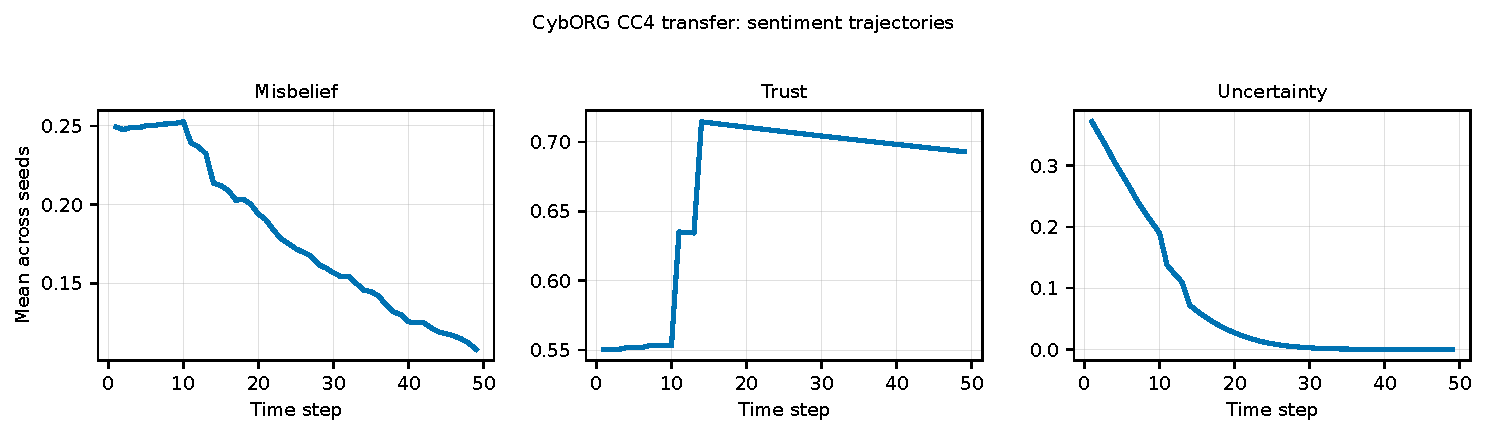
\includegraphics[width=\linewidth]{figures/fig_cyborg_timeseries_grid_gray.pdf}
  \caption{Illustrative CybORG CC4 enterprise transfer run: sentiment trajectories (mean across seeds).}
  \label{fig:cyborg_timeseries}
\end{figure}

\begin{figure}[t]
  \centering
  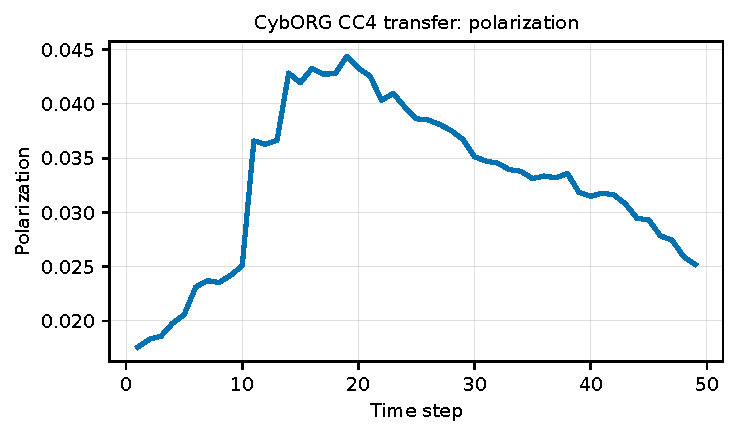
\includegraphics[width=0.8\linewidth]{figures/fig_polarization_cyborg_enterprise_cc4_gray.pdf}
  \caption{Polarization over time for the illustrative CybORG CC4 enterprise transfer run.}
  \label{fig:cyborg_polarization_only}
\end{figure}


%%%%%%%%%%%%%%%%%%%%%%%%%%%%%%%%%%%%%%%%%%
%\isPreprints{}{% This command is only used for ``preprints''.
\begin{adjustwidth}{-\extralength}{0cm}
%} % If the paper is ``preprints'', please uncomment this parenthesis.
%\printendnotes[custom] % Un-comment to print a list of endnotes

\reftitle{References}

% Please provide either the correct journal abbreviation (e.g. according to the “List of Title Word Abbreviations” http://www.issn.org/services/online-services/access-to-the-ltwa/) or the full name of the journal.
% Citations and References in Supplementary files are permitted provided that they also appear in the reference list here. 

%=====================================
% References, variant A: external bibliography
%=====================================
 \bibliography{refs}



% If authors have biography, please use the format below
%\section*{Short Biography of Authors}
%\bio
%{\raisebox{-0.35cm}{\includegraphics[width=3.5cm,height=5.3cm,clip,keepaspectratio]{Definitions/author1.pdf}}}
%{\textbf{Firstname Lastname} Biography of first author}
%
%\bio
%{\raisebox{-0.35cm}{\includegraphics[width=3.5cm,height=5.3cm,clip,keepaspectratio]{Definitions/author2.jpg}}}
%{\textbf{Firstname Lastname} Biography of second author}

% For the MDPI journals use author-date citation, please follow the formatting guidelines on http://www.mdpi.com/authors/references
% To cite two works by the same author: \citeauthor{ref-journal-1a} (\citeyear{ref-journal-1a}, \citeyear{ref-journal-1b}). This produces: Whittaker (1967, 1975)
% To cite two works by the same author with specific pages: \citeauthor{ref-journal-3a} (\citeyear{ref-journal-3a}, p. 328; \citeyear{ref-journal-3b}, p.475). This produces: Wong (1999, p. 328; 2000, p. 475)

%%%%%%%%%%%%%%%%%%%%%%%%%%%%%%%%%%%%%%%%%%
%% for journal Sci
%\reviewreports{\\
%Reviewer 1 comments and authors’ response\\
%Reviewer 2 comments and authors’ response\\
%Reviewer 3 comments and authors’ response
%}
%%%%%%%%%%%%%%%%%%%%%%%%%%%%%%%%%%%%%%%%%%
\PublishersNote{}
%\isPreprints{}{% This command is only used for ``preprints''.
\end{adjustwidth}
%} % If the paper is ``preprints'', please uncomment this parenthesis.
\end{document}

